\section{Sensitivity of LHC measurements to Vector-like Quarks}
\label{sec:VLQ}
Vector-like quarks belong to a separate family than the SM quarks. They are non-chiral, and thus both the left- and right-handed components transofrm the same way under the SM symmetries. This enables them to have a bare mass term and obtain mass without interacting with the Higg boson. Consequently, they are not constrained by Higgs measurements, unlike a fourth generation in the SM quark family. In short, VLQs are simplest example of coloured fermions still allowed by experimental data \cite{Aguilar_Saavedra_2013}. 

Vector-like quarks arise in many classes of BSM theories, such as composite Higgs that assume electroweak symmetry breaking is due to a a new strongly interacting sector~\cite{witzel2019review}, or little Higgs models that introduce extended global symmetries, or models with extra dimensional symmetries \todo{Add some citations for these models}. As with most models extending the SM, many of these introduce new sources of CP violation.

\subsection{Phenomenology of VLQs}
For the material presented in this section, vector-like quarks are studied in a model-independent fashion involving few free parameters. The framework is developed in Reference~\cite{}, which presents an effective Lagrangian description for vector-like quarks that is easily translated to experimental observables. The Lagrangian is written in equation 3.2 of Reference~\cite{} as:
\begin{equation}
  \label{eq:vlqlagr}
  \begin{split}
    \mathcal{L} =
    &  \kappa_B \left[
      \sqrt{\frac{\zeta_i\xi^{B}_{W}}{\Gamma^0_{W}}} \frac{g}{\sqrt{2}} [\bar{B}_{L/R} W^-_\mu \gamma^\mu u^i_{L/R}]
      +  \sqrt{\frac{\zeta_i\xi^{B}_{Z}}{\Gamma^0_{Z}}} \frac{g}{2c_W} [\bar{B}_{L/R} Z_\mu \gamma^\mu d^{\,i}_{L/R}]
      -  \sqrt{\frac{\zeta_i\xi^{B}_{H}}{\Gamma^0_{H}}} \frac{M_B}{v} [\bar{B}_{R/L} H d^{\,i}_{L/R}]
    \right] \\
    + &   \kappa_T \left[
      \sqrt{\frac{\zeta_i\xi^{T}_{W}}{\Gamma^0_{W}}} \frac{g}{\sqrt{2}} [\bar{T}_{L/R} W^+_\mu \gamma^\mu d^{\,i}_{L/R}]
      +  \sqrt{\frac{\zeta_i\xi^{T}_{Z}}{\Gamma^0_{Z}}} \frac{g}{2c_W} [\bar{T}_{L/R} Z_\mu \gamma^\mu u^i_{L/R}]
      -  \sqrt{\frac{\zeta_i\xi^{T}_{H}}{\Gamma^0_{H}}} \frac{M_T}{v} [\bar{T}_{R/L} H u^i_{L/R}]
    \right] \\
    +  &  \kappa_X \left[
      \sqrt{\frac{\zeta_i}{\Gamma^0_{W}}} \frac{g}{\sqrt{2}} [\bar{X}_{L/R} W^+_\mu \gamma^\mu u^i_{L/R}]
    \right]
    + \kappa_Y \left[
      \sqrt{\frac{\zeta_i}{\Gamma^0_{W}}} \frac{g}{\sqrt{2}} [\bar{Y}_{L/R} W^-_\mu \gamma^\mu d^{\,i}_{L/R}]
    \right] + \text{h.c.} \, ,
    % + & \kappa_g \left[ \frac{g_s v}{2\Lambda^2} f_i^{L/R} \bar{Q}_{R/L} G_{\mu\nu}\sigma^{\mu\nu} q^{i}_{L/R} \right] + h.c...
  \end{split}
\end{equation}
where $B$, $T$, $X$, and $Y$ are the four types of vector-like quarks with triplet colour charges, and electromagnetic charges $-\frac{1}{3}$, $\frac{2}{3}$, $\frac{5}{3}$ and $-\frac{4}{3}$ respectively. The couplings with the photon and gluon are derived via the standard gauge invariance route. The overall coupling strength of the vector-like quarks $Q$ are governed by the parameters $\kappa_Q$. $\zeta_i$ represents the coupling of the vector-like quarks to the $i^\text{th}$ generation SM quark. $\xi^B_V$ and $\xi^T_V$ govern the couplings of the $B$ and $T$ quarks to $Z$, $W$, and Higgs bosons via new $QqV$ vertices. Another free parameter is the mass of the new quarks, denoted as $M_Q$. Under the assumption that $\sum_{V} \xi^B_{V} = 1$ and $\sum_{V} \xi^T_{V} = 1$, and $\sum_{i} \zeta_i = 1$, the branching ratio of any vector-like quark to an SM quark and gauge boson is written as
\begin{equation}
    \textrm{BR}(Q \rightarrow Vq_i) = \zeta_i\xi^{V}.
\end{equation}

At the LHC, vector-like quarks can be either pair- or singly-produced. Pair-production occurs via the strong and electromagnetic interaction, and via the weak interaction through the $t$-channel exchange of an SM weak boson. Single production in association with a quark or with an SM boson occurs via the weak interaction only. Examples of leading-order Feynman diagrams for VLQ production are shown in Figure~\ref{fig:feyndiags}. Vector-like quarks can only decay via the weak interaction into an SM weak boson and an SM quark. Given the charge assignments, the possible decay channels of the vector-like quarks are:
\begin{equation}
    B^{-\frac{1}{3}}\rightarrow W^- + q_u, \quad Z + q_d, \quad H + q_d \\
    T^{+\frac{2}{3}}\rightarrow W^+ + q_d, \quad Z + q_u, \quad H + q_u \\
    X^{+\frac{5}{3}}\rightarrow W^+ + q_u \\
    Y^{-\frac{4}{3}}\rightarrow W^- + q_d .
\end{equation}
The $B$ and $T$ quark decays to the $W$, $Z$, or Higgs boson plus an up- or down-type quark, depending on the values of the $\xi^V$ and $\zeta_i$ parameters. The $X$ and $Y$ quarks, however, can only decay via the $W$ decay channel due to electromagnetic charge conservation, and are unaffected by the values of $\xi^V$\footnote{Since $\xi^W$=1 and $\xi^Z=\xi^H=0$ are constants for $X$ and $Y$.}. The production rates of the vector-like quarks depend on the mass $m_Q$, especially for the QCD-dominated pair production~\cite{Buchkremer_2013}. The coupling strength factors $\kappa_Q$ drive the electroweak production cross-sections, which are therefore sensitive to the overall strength of the coupling.
\begin{figure}[t]
  \centering
  \subfloat[]{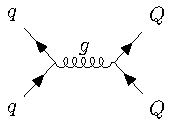
\includegraphics[]{Figures/VLQ/feynmanDiagrams/diagram-5.pdf}\label{fig:feyndiags:QQ1}}
  \subfloat[]{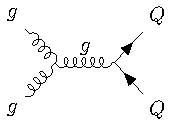
\includegraphics[]{Figures/VLQ/feynmanDiagrams/diagram-9.pdf}\label{fig:feyndiags:QQ2}}
  \subfloat[]{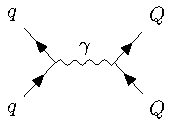
\includegraphics[]{Figures/VLQ/feynmanDiagrams/diagram-6.pdf}\label{fig:feyndiags:QQ3}}\\
  \subfloat[]{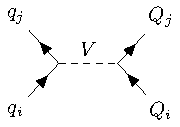
\includegraphics[]{Figures/VLQ/feynmanDiagrams/diagram-8.pdf}\label{fig:feyndiags:QQ'1}}
  \subfloat[]{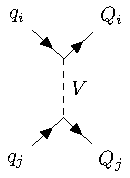
\includegraphics[]{Figures/VLQ/feynmanDiagrams/diagram-7.pdf}\label{fig:feyndiags:QQ'2}}\\ % Valence
  \subfloat[]{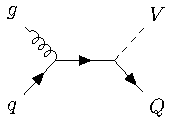
\includegraphics[]{Figures/VLQ/feynmanDiagrams/diagram-1.pdf}\label{fig:feyndiags:QV1}}
  \subfloat[]{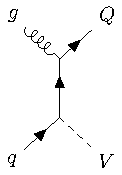
\includegraphics[]{Figures/VLQ/feynmanDiagrams/diagram-2.pdf}\label{fig:feyndiags:QV2}}
  \subfloat[]{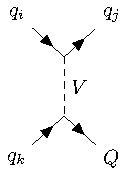
\includegraphics[]{Figures/VLQ/feynmanDiagrams/diagram-3.pdf}\label{fig:feyndiags:Qq1}} % Valence
  \subfloat[]{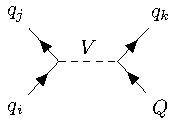
\includegraphics[]{Figures/VLQ/feynmanDiagrams/diagram-4.pdf}\label{fig:feyndiags:Qq2}}
  \caption{Leading-order Feynman diagrams for production of VLQs $Q$.  The top row (\protect\subref*{fig:feyndiags:QQ1}--\protect\subref*{fig:feyndiags:QQ3}) shows VLQ pair-production diagrams via strong and EM interactions, which do not depend on $\kappa$.  The second row (\protect\subref*{fig:feyndiags:QQ'1}--\protect\subref*{fig:feyndiags:QQ'2}) shows pair-production of VLQs via a weak boson $V \in \{W,Z,H\}$, which may lead to different-flavoured VLQs in the final state. The third row (\protect\subref*{fig:feyndiags:QV1}--\protect\subref*{fig:feyndiags:Qq2}) shows single-production of $Q$ in association with a weak boson or SM quark $q$. All Feynman diagrams are taken from Reference~\cite{VLQ_contur}}.
\label{fig:feyndiags}
\end{figure}

The phenomenology of vector-like quark production and decay can be inferred from the Lagrangian of Equation~\ref{eq:vlqlagr}. In particular, the production cross-sections are dependent on $M_Q$ and $\kappa$. For this section, it is assumed that the $B,T,X$, and$Y$ quarks all have the same mass and coupling strength (i.e. $M_B = M_T = M_X = M_Y$ and $\kappa_B = \kappa_T = \kappa_X = \kappa_Y$). 

\subsubsection{Pair production}

Figures~\ref{fig:feyndiags}(\subref*{fig:feyndiags:QQ1}--\subref*{fig:feyndiags:QQ3}) show the pair production of VLQs via the strong and electromagnetic interaction. These three diagrams are not dependent on any of the coupling parameters $\kappa,\xi$ or $\zeta$. For a VLQ of mass
$\sim \unit{1.3}{\TeV}$ at the LHC, the cross-section is of the order of $\unit{10}{\femto\barn}$~\cite{VLQ_contur}. In the second row, Figures~\ref{fig:feyndiags}(\subref*{fig:feyndiags:QQ'1}--\subref*{fig:feyndiags:QQ'2}) show the s- and t-channel pair-production of VLQs through the exchange of a weak boson. These diagrams are dependent on $\kappa$, and may have a non-negligible contribution to the production cross-section. In fact, when the VLQs couple only to first generation SM quarks, Figure~\ref{fig:feyndiags:QQ'2} can become the dominant production mechanism. Since the up and down quarks are the constituents of the proton, Figure~\ref{fig:feyndiags:QQ'2} is the only possible diagram with two incoming valence quarks. All other diagrams require at least one anti-quark or gluon. If the VLQs couple to the second or third generation SM quarks, however, Figure~\ref{fig:feyndiags:QQ'2} is no longer dominant. This effect is illustrated in Figure~\ref{fig:TTproduction} for $TT$ pair-production. For VLQs coupling to the first generation, a dependence on $\kappa$ becomes visible as the mass of the VLQs increase. This feature is not visible for couplings to the second and third generation. The VLQs are produced in pairs of different flavours when mediated by a $W$ boson. For the $X$ and $Y$, this is always the case since they do not couple to the $Z$ or the Higgs. 
\begin{figure}[tbp]
\vspace{-0.4cm}
\subfloat[$T$ coupling to $u,d$ only]{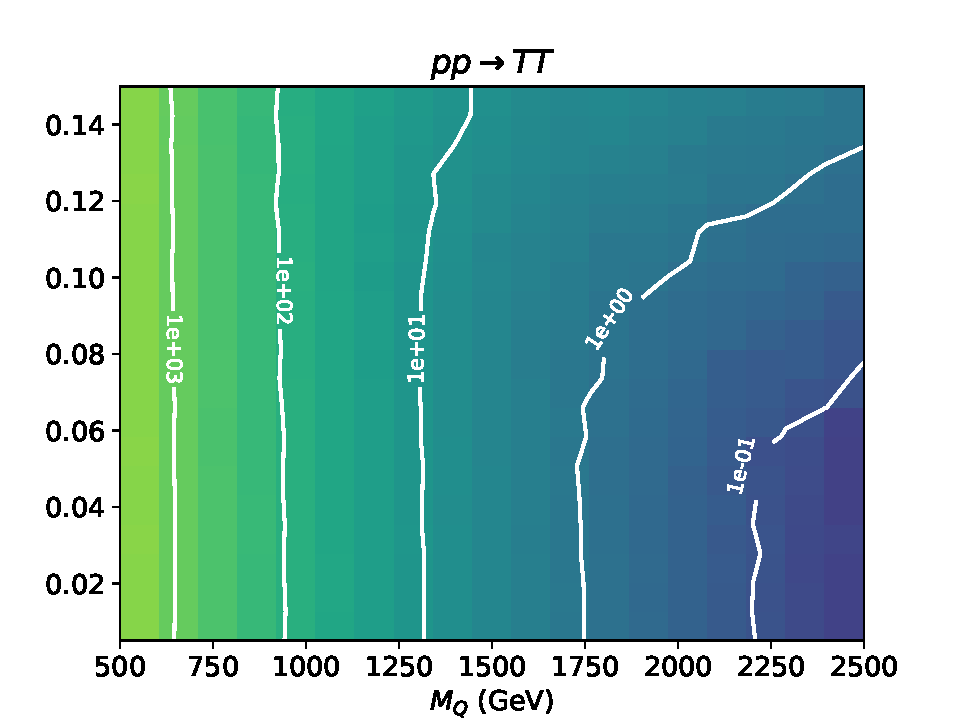
\includegraphics[width=0.33\textwidth]{Figures/VLQ/xsScans/1stGen/p_p____T_T.pdf}} %5000 fb
\subfloat[$T$ coupling to $c,s$ only]{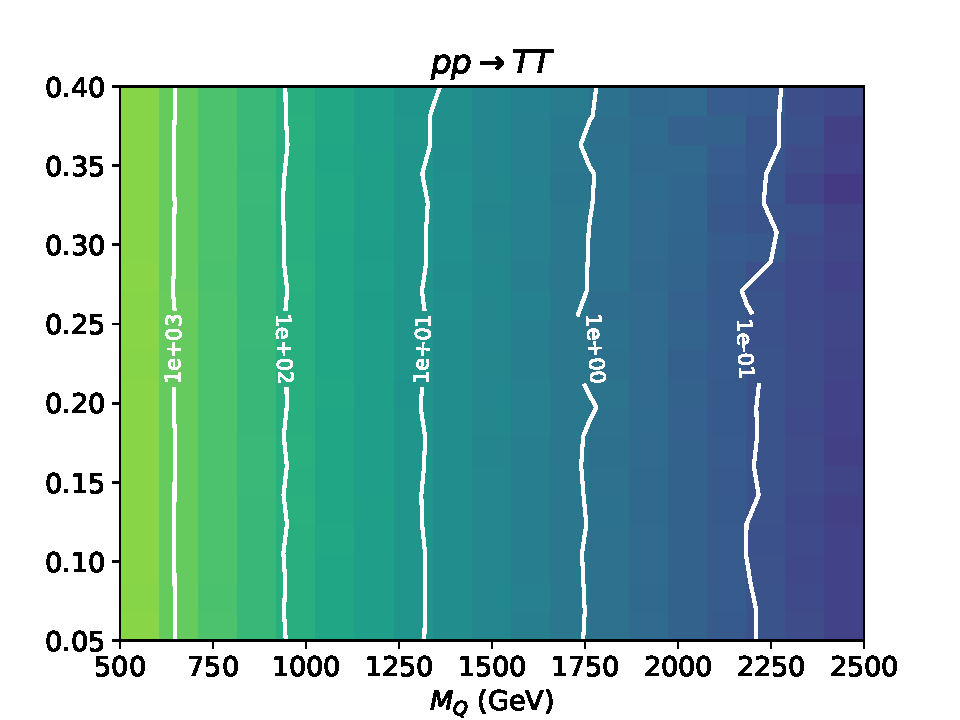
\includegraphics[width=0.33\textwidth]{Figures/VLQ/xsScans/2ndGen/p_p____T_T.pdf}} %5000 fb\\
\subfloat[$T$ coupling to $t,b$ only]{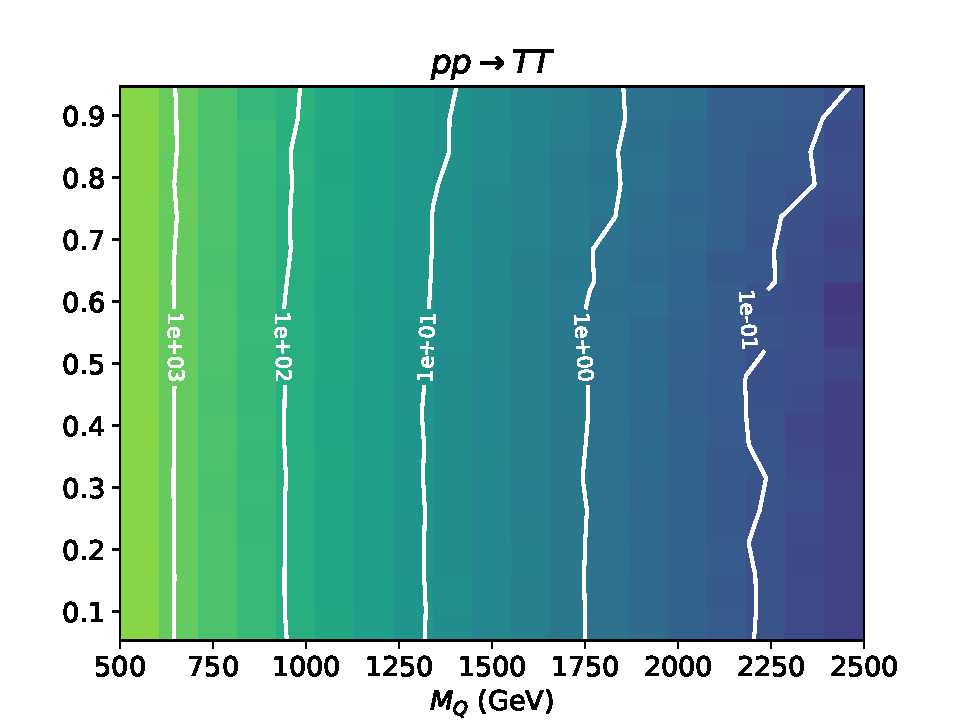
\includegraphics[width=0.33\textwidth]{Figures/VLQ/xsScans/3rdGen/p_p____T_T.pdf}}
\includegraphics[height=3.5cm]{xsScans/3rdGen/cbar.pdf} %5000 fb
\caption{Leading-order cross-sections extracted from Herwig for production of a $TT$ pair as a
  function of $M_Q$ and $\kappa$, for \unit{13}{\TeV} $pp$ collisions, in the
  $\WZH = \WZHtoo$ scenario, assuming couplings to individual generations of
  quarks.  The white lines indicate the contours for production cross-sections
  in multiples of 10. The first-generation cross-sections acquire a dependence
  on $\kappa$ since pair-production initiated by proton valence quarks becomes
  possible.  The situation is analogous for other VLQ flavours, although
  somewhat attenuated for $X$ and $Y$ since they still require at least one
  antiquark from the sea to be produced via $W$ exchange in the $t$-channel. Figure taken from Reference~\cite{VLQ_contur}.}
\label{fig:TTproduction}
\end{figure}

\subsubsection{Single production}
Single production is illustrated in the last row of Figure~\ref{fig:feyndiags}. It can occur in association with a weak boson $V$, or with a Standard Model quark $q$. In both cases a strong $\kappa$ dependence is present since single production always takes place via the weak interaction. 

Looking first at VLQ production alongside a weak boson, it is important to note the dependence of the production cross-section on the flavour of the incoming quark. Consider VLQs that couple only to first generation SM quarks. Using Figures~\ref{fig:feyndiags}(\subref*{fig:feyndiags:QV1}--\subref*{fig:feyndiags:QV2}) one can deduced that $g + u \rightarrow T+H/Z$ production is roughly two times $g + d \rightarrow B+H/Z$ production, due to the composition of the proton's valence quarks, $uud$. Similarly, $g + u \rightarrow B+W$ production is twice as frequent as  $g + d \rightarrow T+W$, and the $g + u \rightarrow X+W$ production cross-section surpasses that of $g + u \rightarrow Y+W$. Factoring in the weak boson couple ratio of  $\WZH = \WZHtoo$, the dominant production process is $X+V$. The $B+V$ and $T+V$ production rates are 25\% less frequent, and $Y+V$ is 50\% less frequent. When VLQs couple to the second or third generation SM quarks, the valence quark effect disappears and single-production is suppressed compared to pair-production. In the case of third-generation coupling, diagrams that include a top quark are nearly vanish. $X+W$, $T+H/Z$, and $B+W$ production becomes largely impossible. These effects are illustrated in Figure 3 of Reference~\cite{VLQ_contur} and reproduced in Figure~\ref{fig:QVproduction}. Shown is the production cross-sections for $T+V$ and $Y+V$ for VLQs coupling to first-, second- or third-generation SM quarks. 

\begin{figure}[t]
    \vspace{-0.4cm}
    \subfloat[$T$ coupling to $u,d$ only]{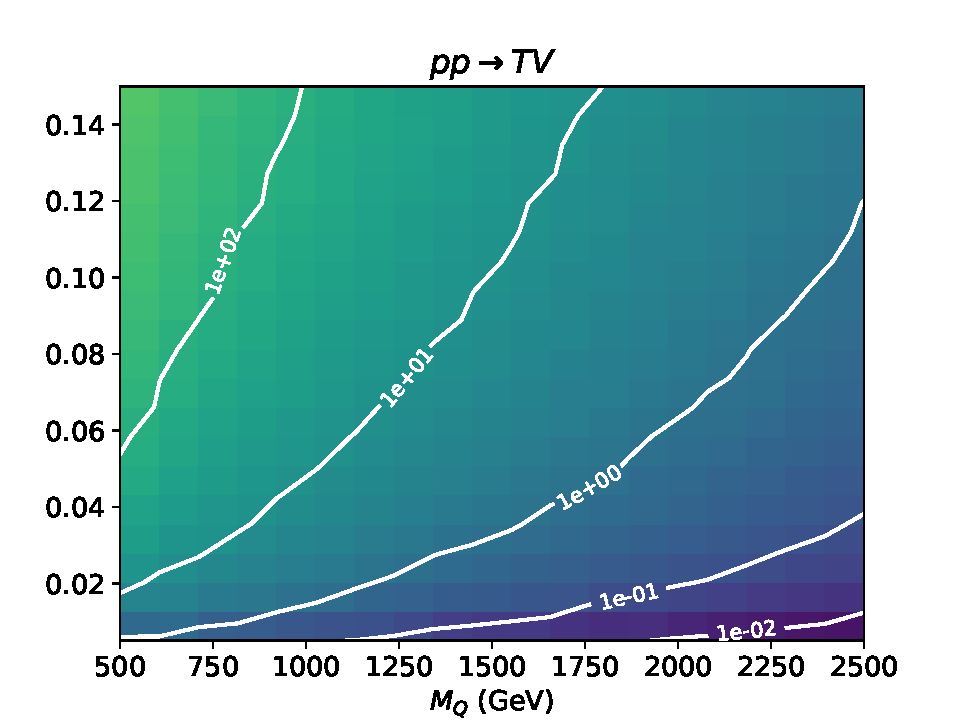
\includegraphics[width=0.33\textwidth]{Figures/VLQ/xsScans/1stGen/p_p____T_V.pdf}} %5000 fb
    \subfloat[$T$ coupling to $c,s$ only]{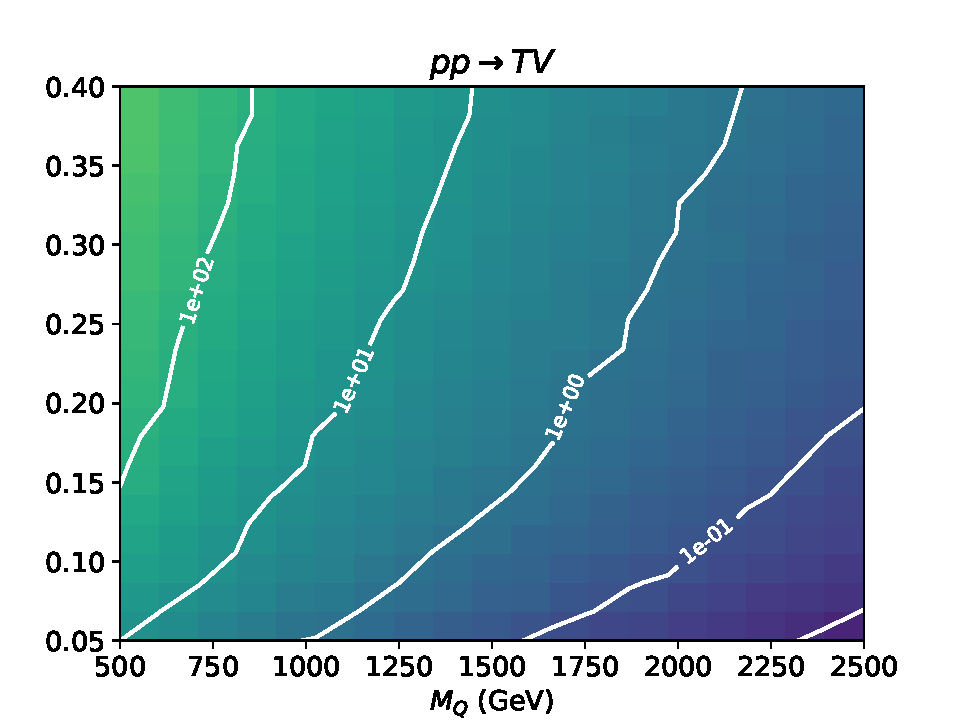
\includegraphics[width=0.33\textwidth]{Figures/VLQ/xsScans/2ndGen/p_p____T_V.pdf}} %5000 fb\\
    \subfloat[$T$ coupling to $t,b$ only]{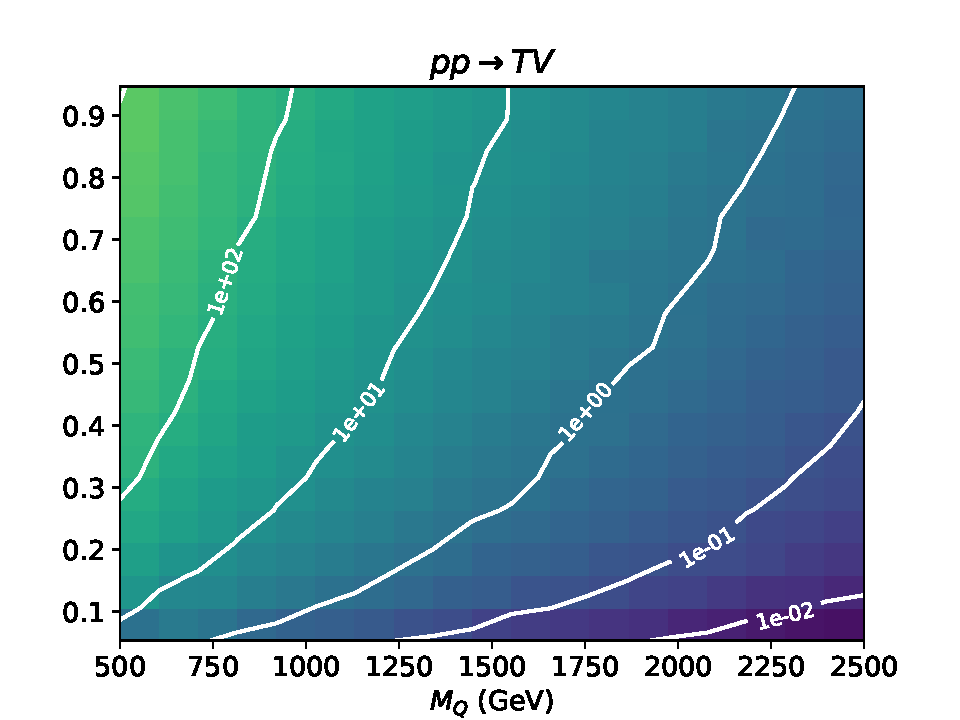
\includegraphics[width=0.33\textwidth]{Figures/VLQ/xsScans/3rdGen/p_p____T_V.pdf}} %5000 fb
    \includegraphics[height=3.5cm]{xsScans/3rdGen/cbar.pdf} %5000 fb\\
    \subfloat[$Y$ coupling to $u,d$ only]{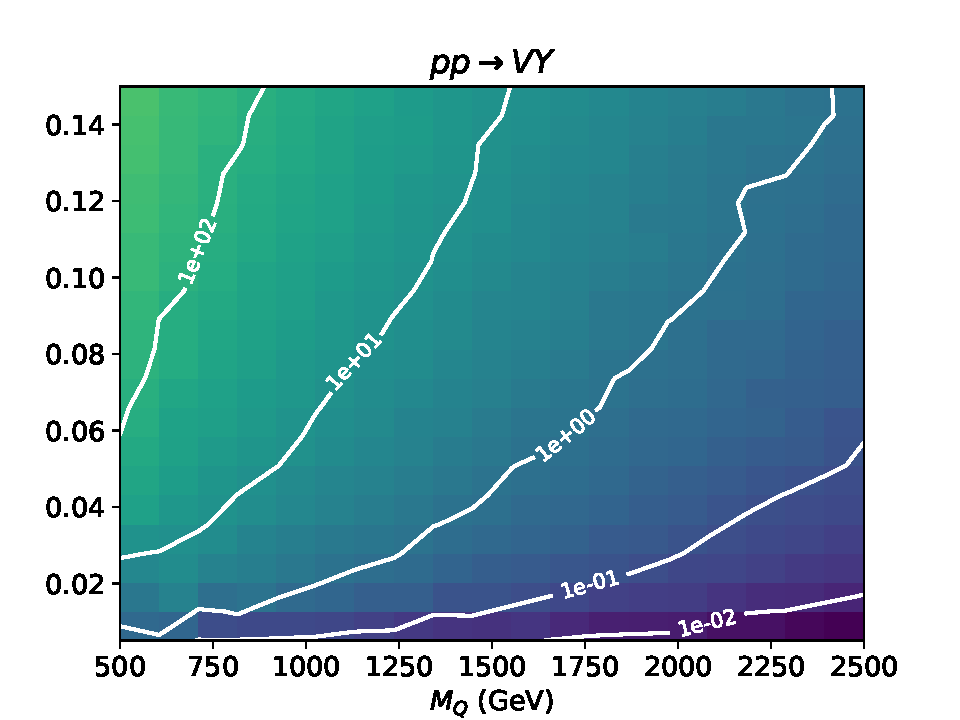
\includegraphics[width=0.33\textwidth]{Figures/VLQ/xsScans/1stGen/p_p____V_Y.pdf}} %5000 fb
    \subfloat[$Y$ coupling to $c,s$ only]{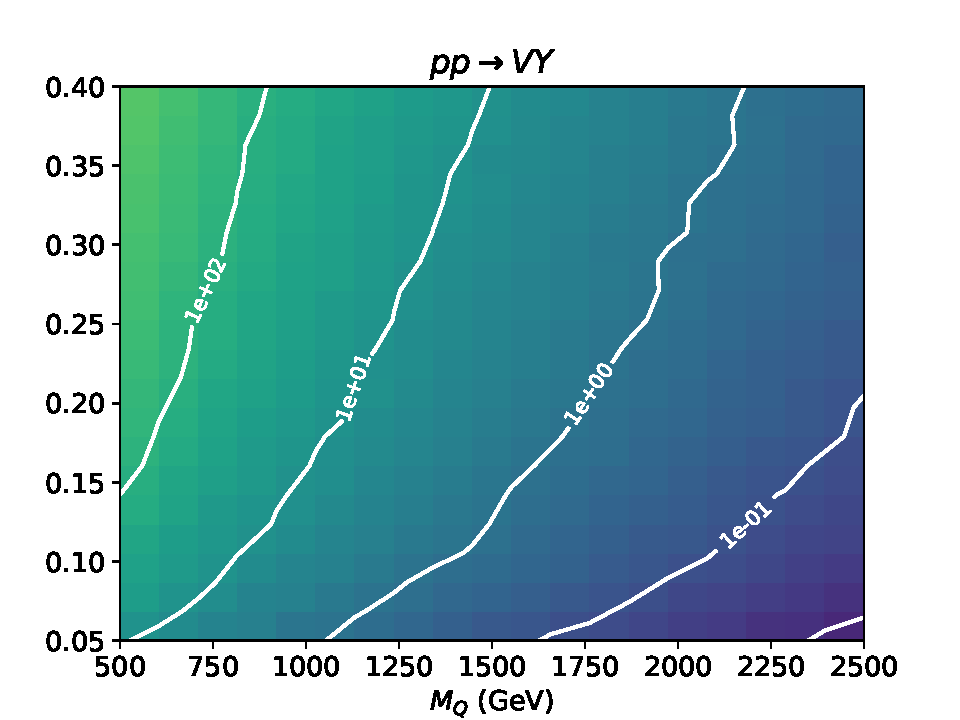
\includegraphics[width=0.33\textwidth]{Figures/VLQ/xsScans/2ndGen/p_p____V_Y.pdf}} %5000 fb\\
    \subfloat[$Y$ coupling to $t,b$ only]{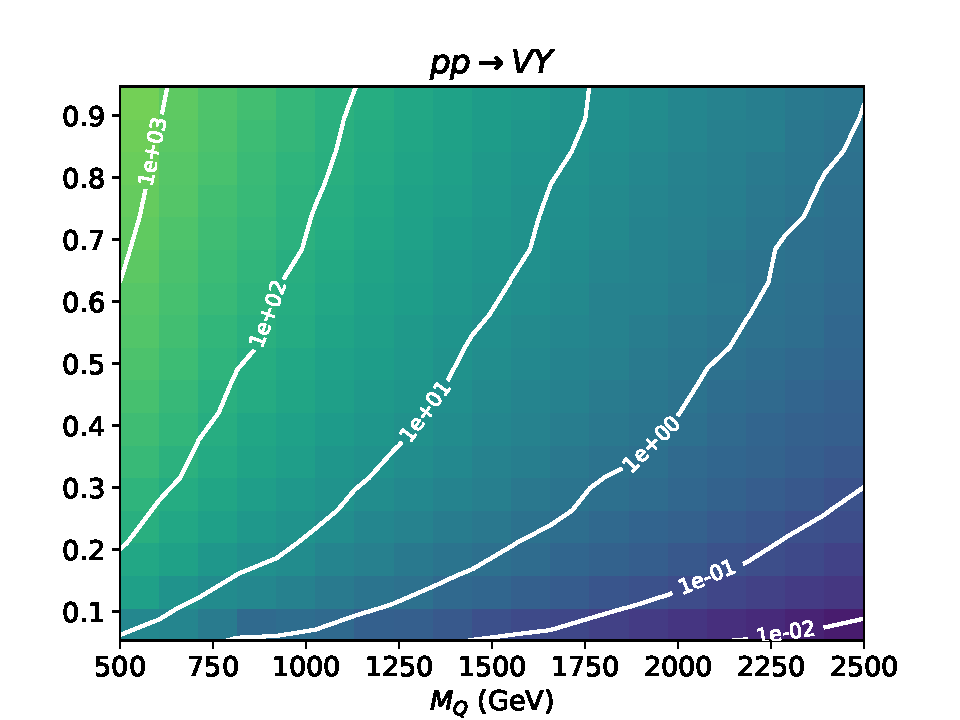
\includegraphics[width=0.33\textwidth]{Figures/VLQ/xsScans/3rdGen/p_p____V_Y.pdf}} %5000 fb
    \includegraphics[height=3.5cm]{xsScans/3rdGen/cbar.pdf} %5000 fb
    \caption{Leading-order cross-sections extracted from Herwig for production of a $T$ and $Y$
      with a weak boson as a function of $M_Q$ and $\kappa$, for \SI{13}{\TeV} $pp$
      collisions, in the $\WZH = \WZHtoo$ scenario, assuming couplings to individual
      generations of quarks.  The white lines indicate the contours for production
      cross-sections in multiples of 10. First-generation couplings lead to higher
      production cross-sections, as a result of valence-quark-induced diagrams,
      while second and third-generation couplings lead to suppressed production
      rates, according to the relevant quark PDFs. Figure taken from Reference~\cite{VLQ_contur}.}
    \label{fig:QVproduction}
\end{figure}
Figures~\ref{fig:feyndiags}(\subref*{fig:feyndiags:Qq1}--\subref*{fig:feyndiags:Qq2}) show the single-production of VLQs in association with a quark, mediated by a weak boson. Considering the case where VLQs couple to first-generation quarks, the dominant production mechanism is the $t-$channel diagram where both the incoming quarks can be valence quarks. Valence quarks, on average, carry a larger portion of the proton's momentum than sea quarks. Diagrams with $dd$ induced VLQ production have the lowest cross-section, and $ud$ or $uu$ induced cross-sections are four times higher~\footnote{Since the proton composition is $uud$, the possible incoming quark pairs are: $uu, uu, ud,$; $uu, uu, ud,$; $du, du,$ and $dd$.}. Consequently, the dominant production process is $u + u \rightarrow X + q$, which is four times as frequent as the $dd$ induced $Y + q$. Both are mediated by a $W$ boson. For $B + q$ and $T + q$ production there is a further suppression from the small coupling of the Higgs boson to light SM quarks. When the VLQs couple to the second-generation quarks, the production cross-sections are dependent on the quark PDFs. For coupling to the third-generation, some production modes are inaccessible if they involve an incoming top quark. This effect is illustrated in Figure 4 of Reference~\cite{VLQ_contur} and reproduced in Figure~\ref{fig:Qqproduction}, where the production cross-sections for $T$ and $X$ in association with a quark are illustrated.
\begin{figure}[tbp]
    \vspace{-0.4cm}
    \subfloat[$T$ coupling to $u,d$ only]{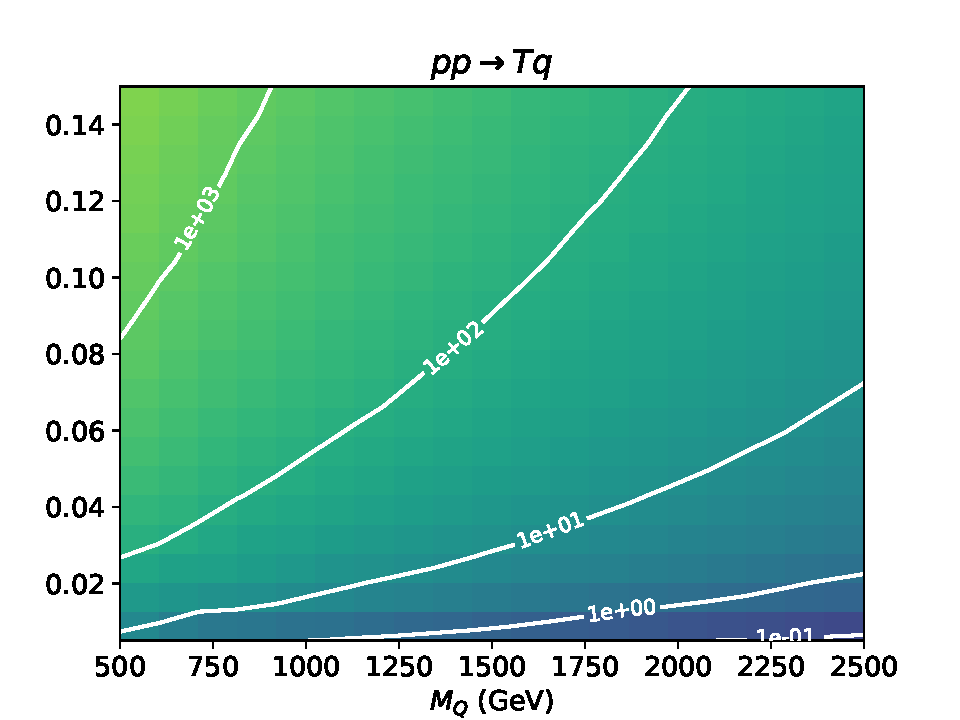
\includegraphics[width=0.33\textwidth]{Figures/VLQ/xsScans/1stGen/p_p____T_q.pdf}} %5000 fb
    \subfloat[$T$ coupling to $c,s$ only]{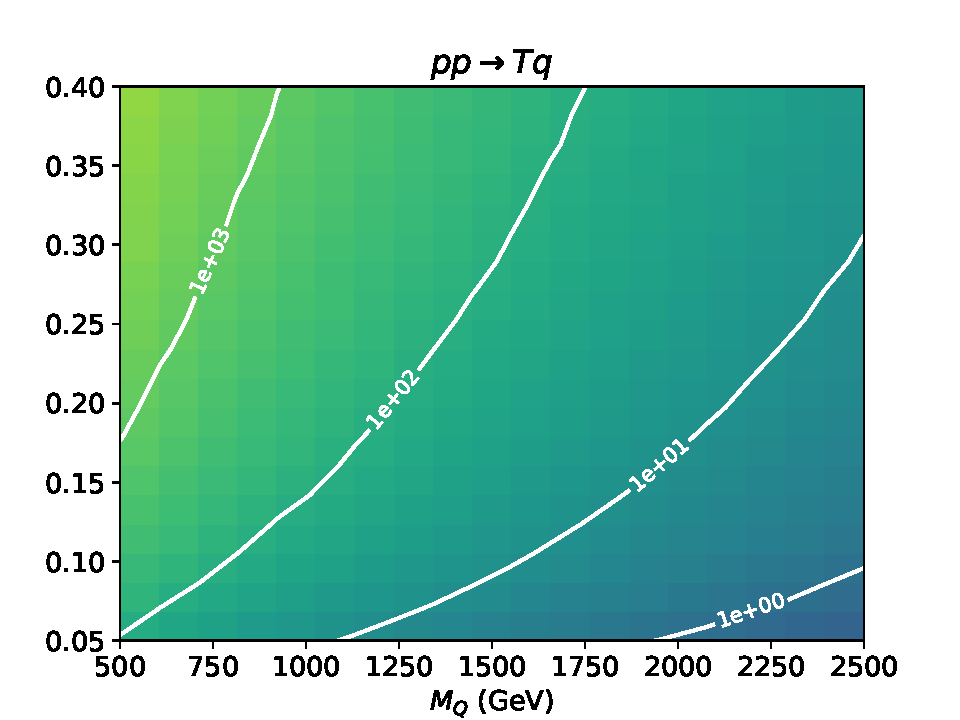
\includegraphics[width=0.33\textwidth]{Figures/VLQ/xsScans/2ndGen/p_p____T_q.pdf}} %5000 fb\\
    \subfloat[$T$ coupling to $t,b$ only]{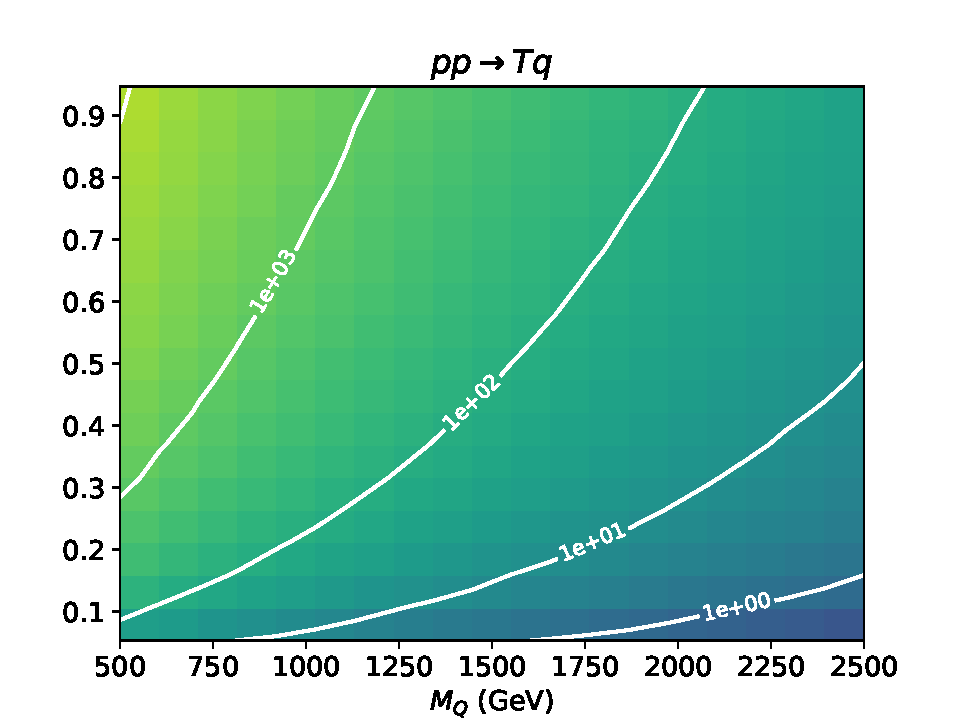
\includegraphics[width=0.33\textwidth]{Figures/VLQ/xsScans/3rdGen/p_p____T_q.pdf}} %5000 fb
    \includegraphics[height=3.5cm]{xsScans/3rdGen/cbar.pdf} %5000 fb \\
    \subfloat[$X$ coupling to $u,d$ only]{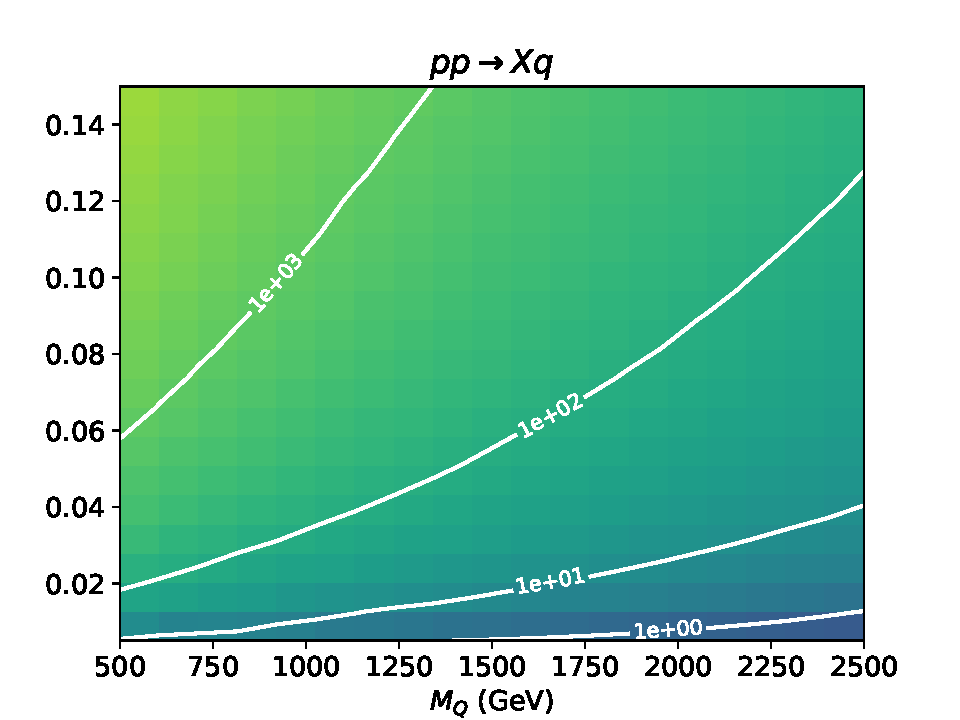
\includegraphics[width=0.33\textwidth]{Figures/VLQ/xsScans/1stGen/p_p____X_q.pdf}} %5000 fb
    \subfloat[$X$ coupling to $c,s$ only]{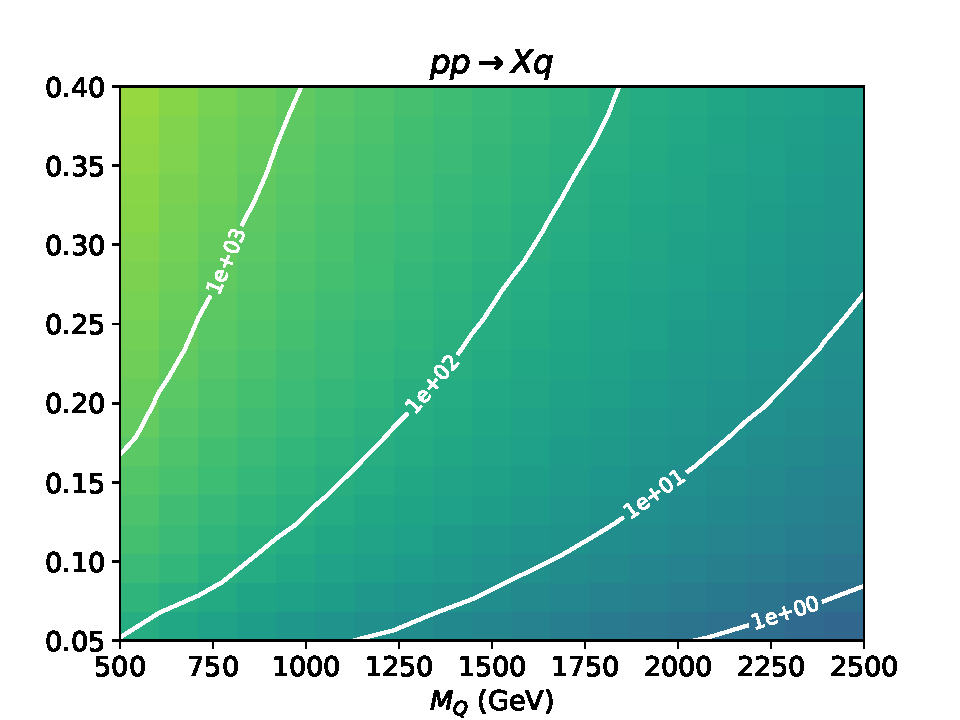
\includegraphics[width=0.33\textwidth]{Figures/VLQ/xsScans/2ndGen/p_p____X_q.pdf}} %5000 fb\\
    \subfloat[$X$ coupling to $t,b$ only]{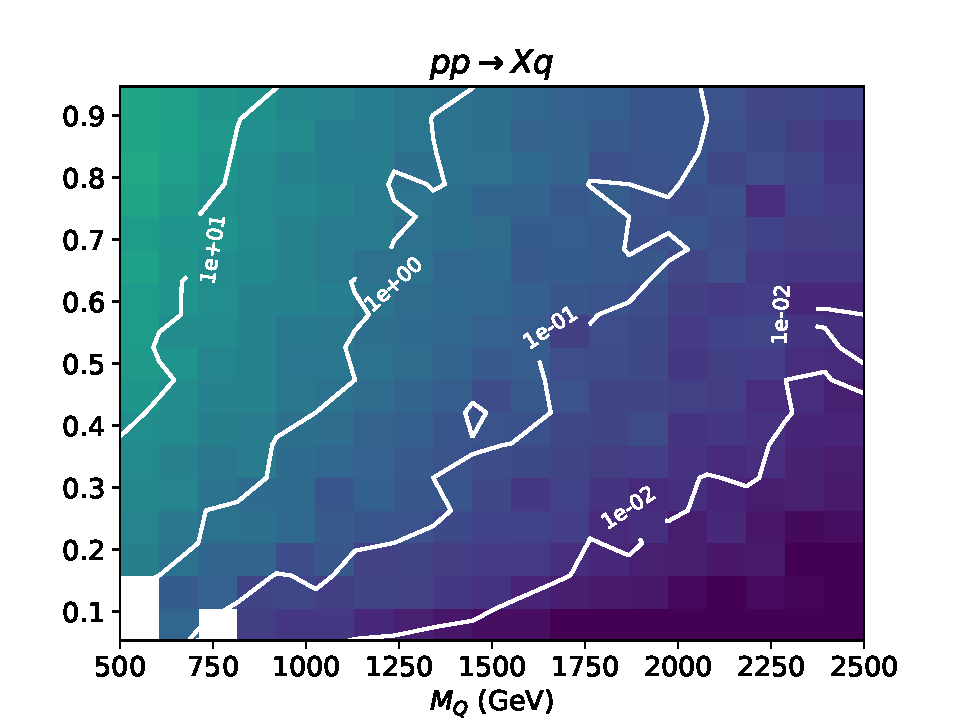
\includegraphics[width=0.33\textwidth]{Figures/VLQ/xsScans/3rdGen/p_p____X_q.pdf}} %5000 fb
    \includegraphics[height=3.5cm]{Figures/VLQ/xsScans/3rdGen/cbar.pdf} %5000 fb
    \caption{Leading-order cross-sections extracted from Herwig for production of a $T$ and $X$
      with a SM quark as a function of $M_Q$ and $\kappa$, for \SI{13}{\TeV} $pp$
      collisions, in the $\WZH = \WZHtoo$ scenario, assuming couplings to individual
      generations of quarks.  The white lines indicate the contours for production
      cross-sections in multiples of 10. First-generation couplings lead to higher
      production cross-sections, as a result of valence-quark-induced diagrams,
      while second and third-generation couplings lead to suppressed production
      rates, according to the relevant quark PDFs. $X+q$ production goes from being
      the dominant production process at the LHC if $X$ couples to first-generation
      quarks only, to vanishing if $X$ couples to third-generation quarks only.
      White cells indicate corners of phase-space where the process in question is highly subdominant, and therefore where the cross-section was not sampled during the Herwig run. Figure taken from Reference~\cite{VLQ_contur}.}
    \label{fig:Qqproduction}
\end{figure}

\subsection{Comparison to \ATLAS searches}
Typically, searches conducted by the \ATLAS and \CMS experiments focus on the $T$ and $B$ vector-like quarks that couple only with the third generation SM quarks. In this sub-section the same assumption are made in order to compare the exclusions from \LHC results to exclusions computed by \contur. The $B$ and $T$ quarks are studied separately with all other VLQs decoupled from the SM. The possible decay channels are $b + Z$, $b + H$ and $t + W$ for the $B$ quark, and similarly $t + Z$, $t + H$ and $b = W$ for the $T$. Both \ATLAS and \CMS have conducted searches targeting specific final states~\todo{Provide some paper citations?}. \ATLAS published a combination limit from multiple searches of pair-produced VLQs in Reference~\cite{ATLAS_VLQ_combination}, and similarly from \CMS in Reference~\cite{Sirunyan_2018}. The \ATLAS results presents the exclusion limits in a two-dimensional parameter space of the VLQ branching ratios which is easily mimicked by \contur.
\begin{figure}[tbp]
    \vspace{-0.4cm}
    \subfloat[]{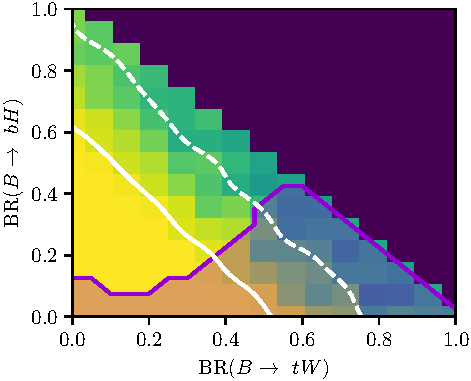
\includegraphics[width=0.45\textwidth]{Figures/VLQ/B/1200/combinedOverlay}\label{fig:BTonlyB}}
    \subfloat[]{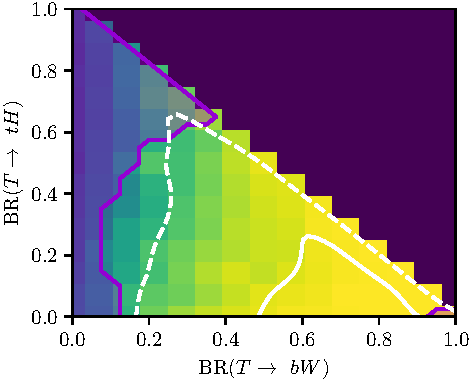
\includegraphics[width=0.45\textwidth]{Figures/VLQ/T/1350/combinedOverlay}\label{fig:BTonlyT}}
    \caption{Sensitivity of LHC measurements to
    \protect\subref{fig:BTonlyB}~$B$-production for $M_B = \SI{1200}{\GeV}$ and
    \protect\subref{fig:BTonlyT}~$T$-production for $M_T = \SI{1350}{\GeV}$.
    The \contur exclusion is shown in the bins in which it is evaluated,
    graduated from yellow through green to black on a linear scale, with the 95\%~CL (solid white)
    and 68\%~CL (dashed white) exclusion contours superimposed. The mauve region
    is excluded at 95\%~CL by the ATLAS combination~\cite{Aaboud:2018pii}.}
    \label{fig:BTonly}
\end{figure}

Figures~\ref{fig:BTonlyB} and~\ref{fig:BTonlyT} show the results of the \contur scan in the triangular plane of the branching ratios to the weak bosons, for $M_B = \unit{1200}{\GeV}$ and $M_T = \unit{1350}{\GeV}$ respectively. It is assumed that the sum of the branching ratios to the $W$, $Z$, and Higgs bosons is equal to one. On the $x$-axis is the BR to $W$'s $\xi^W$, and on the $y$-axis is $\xi^H$. The branching ratio to $Z$ bosons, therefore, is $1-\xi^W-\xi^H$. The shaded purple region shows the excluded phase-space at 95\% confidence level (CL) by \ATLAS. 

Looking first at Figure~\ref{fig:BTonlyB} for the VLB, the excluded region from \contur is in the $Z$ corner of the branching ratio triangle and comes mainly from $Z+$jet measurements~\cite{Aad:2015auj,Aaboud:2017hox,Aaboud:2017hbk,Aaboud:2019jcc}. tHE \ATLAS limit in mauve, on the other hand, receives contributions from four main searches: one each targeting the $Z$ and $H$ decay channels~\cite{ZllSearch,HadSearch}, and the remaining two target $B$-decay to $Wt$~\cite{WtSearch,TriLepSearch}. As a result, the sensitivity for $BR(B\rightarrow tW)$ is high, thus leading to a strong exclusion at the bottom-right corner of the triangle. The excluded regions from \contur and \ATLAS are somewhat complementary. 

Show in Figure~\ref{fig:BTonlyT} is the excluded region from \contur for
$M_T = \SI{1350}{\GeV}$, and the \ATLAS search exclusion for this mass value in mauve. Here there are three analyses going into to the \ATLAS combination limit which target $T$-decay to $Ht$~\cite{HbbSearch,TriLepSearch,HadSearch}, two that target $T$-decay to $Zt$~\cite{ZnunuSearch,ZllSearch}, and only one sensitive in the $W$ channel~\cite{WbSearch}. The \ATLAS sensitivity is mainly in the Higgs corner of the branching ratio half-plane. In contrast, the \contur exclusion comes mainly from top quark and $W$ boson measurements~\cite{Aaboud:2017fye,Aaboud:2018eqg,Sirunyan:2018wem,Khachatryan:2016mnb,Sirunyan:2018ptc}, giving sensitivity in the $W$ corner. The complementarity between \contur and direct searches is nicely demonstrated. 

\subsection{All quark generations}
Although most searches at \ATLAS and \CMS assume that VLQs couple only to the third-generation quarks, it is not at all the case that mixing with the first- and second-generation quarks are forbidden. They do, however, receive more stringent lower bounds on the overall coupling $\kappa$ from flavour physics~\cite{Buchkremer_2013}. These bounds come from the LEP measurements of the $Z$ boson's couplings to light quarks, and from other low energy experiments such as the measurement of the weak charge of the Cesium atom (Atom Parity Violation)~\cite{}. These measurements are proportional to the branching fraction to the specific generation, and therefore from it an absolute bound on $\kappa$ can be extracted. For VLQs that couple only to one SM quark generation at a time, these bounds are estimated to be$\kappa<0.07$ and $\kappa=0.2$ for coupling to the first- and second-generation only. Although scenarios with VLQ couplings to all generations is allowed, they suffer from an extra order of magnitude suppression on $\kappa$~\cite{}. 

At low VLQ masses, the QCD induced pair production mode is dominant. As previously discussed, this is independent of the overall coupling $\kappa$. However, pair production sees a suppression from PDF rescaling at high VLQ masses, therefore when $M_Q$ is large enough, single production becomes dominant~\cite{Panizzi:2014dwa}. This feature is of particular interest when the VLQs couple to first-generation quarks. Since the proton's valence quarks are of the first-generation, production diagrams that involve two incoming initial state quarks will see an enhancement. In particular, the $t-$channel VLQ pair production via the weak interaction (Figure~\ref{}) becomes dominant, and a dependence on $kappa$ comes into play. 
The rest of this subsection explores the VLQs coupling to each of the SM quark generations independently, in four $\xi_V$ branching fraction scenario indicated by ratios: 
\begin{itemize}
	\item{$W:H:Z=0:0:1$ coupling only to the $Z$ boson}
	\item{$W:H:Z=0:1:0$ coupling only to the Higgs boson}
	\item{$W:H:Z=1:0:0$ coupling only to the $W$ boson}
	\item{$W:H:Z=\frac{1}{2}:\frac{1}{4}:\frac{1}{4}$ an admixture of the three bosons}.
\end{itemize}
The results are presented as two-dimensional exclusion maps in the plane of $M_Q$ and $\kappa$. Each square on the map represents a scan point for a specific $(M_Q,\kappa)$ combination where a CLs value is calculated by \contur. The colour of the square indicates the dominant analyses pool contributing towards the exclusion. The final state of the \ATLAS analysis present in Section~\ref{sec:m4l} is four leptons, and therefore belongs to the four lepton pool in pink. The solid white line is the exclusion at 95\% CLs, and the dashed at 68\%. 

\subsubsection{Coupling to first-generation quarks}
\begin{figure}[tbp]
  \centering
  \subfloat[]{
    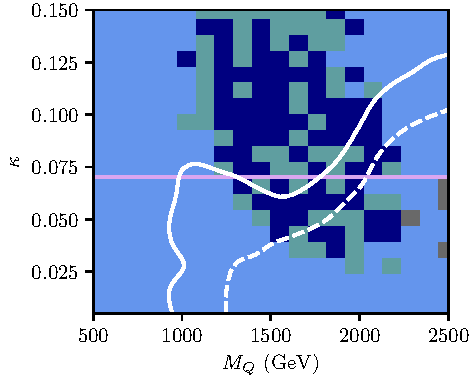
\includegraphics[width=0.45\textwidth]{Figures/VLQ/1Gen/HWZ100/dominantPools0}\label{fig:gen1:001:dom}}
  \subfloat[]{
    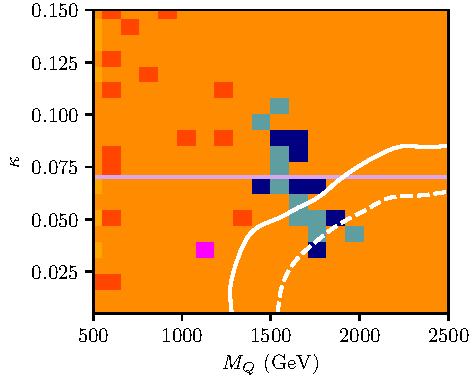
\includegraphics[width=0.45\textwidth]{Figures/VLQ/1Gen/HWZ001/dominantPools0}\label{fig:gen1:010:dom}} \\
  \subfloat[]{
    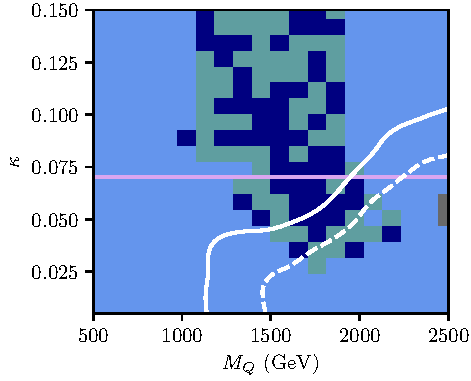
\includegraphics[width=0.45\textwidth]{Figures/VLQ/1Gen/HWZ010/dominantPools0}\label{fig:gen1:100:dom}}
  \subfloat[]{
    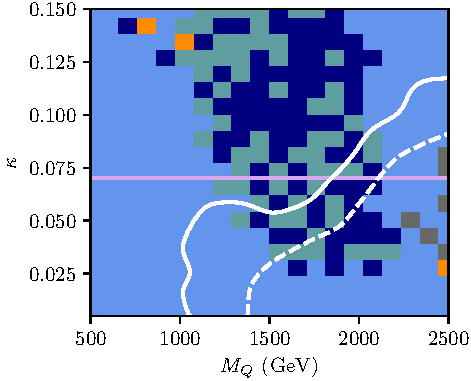
\includegraphics[width=0.45\textwidth]{Figures/VLQ/1Gen/HWZ121/dominantPools0}\label{fig:gen1:121:dom}}
  \vspace*{2ex} \\
  \begin{tabular}{lll}
    \swatch{cornflowerblue}~ATLAS $WW$ & \swatch{navy}~ATLAS $\mu$+\MET{}+jet & \swatch{cadetblue}~ATLAS $e$+\MET{}+jet\\
    % \swatch{gold}~ATLAS $\gamma$
    \swatch{darkorange}~ATLAS $\mu\mu$+jet & \swatch{orangered}~ATLAS $ee$+jet & \swatch{orange!60}~ATLAS $\ell\ell$+jet\\
    % \swatch{orangered!90}~ATLAS $ee$+jet
    \swatch{silver}~ATLAS jets & \swatch{dimgrey}~CMS jets & \\
    \swatch{deepskyblue} CMS~$e$+\MET{}+jet & \swatch{magenta} ATLAS~4$\ell$ &
  \end{tabular}
  \vspace*{2ex}
  \caption{Dominant LHC analysis pools contributing to VLQ limit-setting in the
    $\kappa$ vs VLQ mass plane, where $\kappa$ is the coupling to
    first-generation SM quarks.  All VLQ ($B, T, X, Y$) masses are set to be
    degenerate. The disfavoured regions are located above and to the left of the
    dashed (68\%~CL) and solid (95\%~CL) white contours respectively. The lower
    bounds in $\kappa$ from non-LHC flavour physics are indicated with the pink
    horizontal contour. The VLQ branching fractions to \WZH are
    \protect\subref{fig:gen1:001:dom}~\WZHzzo
    \protect\subref{fig:gen1:010:dom}~\WZHzoz
    \protect\subref{fig:gen1:100:dom}~\WZHozz and
    \protect\subref{fig:gen1:121:dom}~\WZHtoo.}
  \label{fig:1gen:dom}
\end{figure}

The exclusion maps for VLQs coupling to first-generation SM quarks in the four $WHZ$ branching fraction scenarios are show in Figure~\ref{fig:1gen:dom}. The range in $\kappa$ values is from $\kappa=0$ to $\kappa=0.15$. The bound from flavour physics at $\kappa=0.07$ is drawn in pink. In the Higgs only and the mixture scenarios, the $M_Q<1000$~GeV region is largely excluded at 95\% CL. For the $W$ only and $Z$ only configurations, this goes up to $M_Q<1125$~GeV and $M_Q<1250$~GeV respectively. Below these masses the white contour lines are relatively vertical and therefore independent of $\kappa$. This is attributed to the fact that the VLQs are mainly pair-produced via the strong and electromagnetic interaction. Above these masses the contour lines become nearly horizontal, indicating that a strong dependence on $\kappa$ has developed as dominant production mode switches to single production via the weak interaction. Overall the limits at high mass oscillate around $\kappa\sim 0.07$. They are most stringent for the $Z-$only $\xi$ configuration. 

The colouring of the plot indicates the dominant analyses contributing to the exclusion. For all but the $Z$ configuration where $Z+$jets measurements hold the most exclusion power, it is the \ATLAS $WW$ pool in light blue that prevails. This pool contains final state signatures typical of a leptonic $WW$ decay; with two leptons (either $e$ or $\mu$), missing energy $E_T$, and sometimes jets. The sensitivity in the Higgs only corner occurs as a result of the the $H\rightarrow WW$ decay channel. In the middle region of of the Higgs only and $W$ only configuration, there is a strong presence from \ATLAS lepton+\MET{}+jet analyses. This signature is sensitive to the weakly and singly produced VLQ, thus introducing a reliance on $\kappa$ and driving the exclusion contour horizontally. Multiple measurements contribute to each analyses pool. An investigation into the appearance of the lepton+\MET{}+jet pool reveals that it is dominated by measurements of leading jet \pT in the detector-corrected control regions of the \unit{8}{\TeV} \ATLAS vector-boson fusion (VBF) $Wjj$ analysis~\cite{Aaboud:2017fye}. In the \unit{1}{\TeV}-\unit{2}{\TeV} range, the VLQ decays shows up as an excess in the highest leading jet \pT bin. This is illustrated in Figure~\ref{} for the $W$ only configuration at $M_Q=\unit{1000}{\GeV}$, \unit{1750}{\GeV}, and \unit{2250}{\GeV}. These are excluded at 28\%, 91\%, and 41\% respectively. For higher masses the enhancement is out of bin range, and the cross-section also drops. 

\begin{figure}[th]
  \centering
  % \rule{10em}{8em} \quad \rule{10em}{8em} \quad \rule{10em}{8em}\\[1em]
  \hspace*{-3.5em}%
  \mbox{%
    \subfloat[]{
      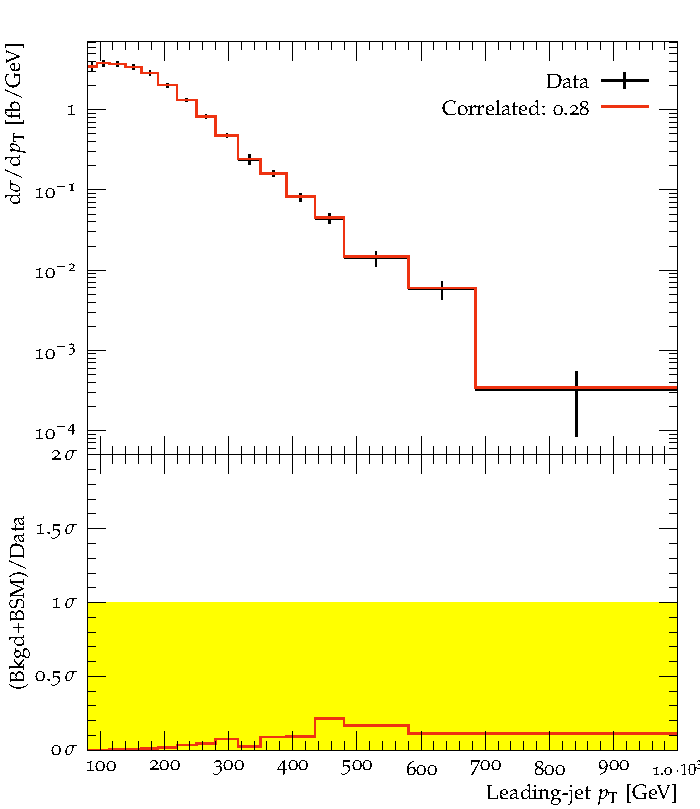
\includegraphics[width=0.36\textwidth]{Figures/VLQ/1Gen/HWZ010/Rivet/0105/d75-x01-y01}\label{fig:gen1:wjjscan:a}}
    \quad
    \subfloat[]{
      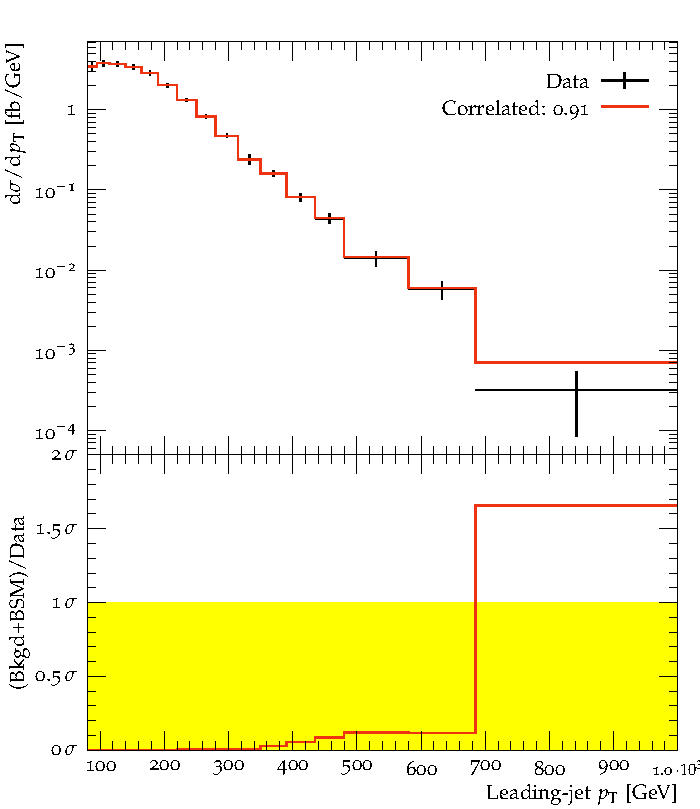
\includegraphics[width=0.36\textwidth]{Figures/VLQ/1Gen/HWZ010/Rivet/0152/d75-x01-y01}\label{fig:gen1:wjjscan:b}}
    \quad
    \subfloat[]{
      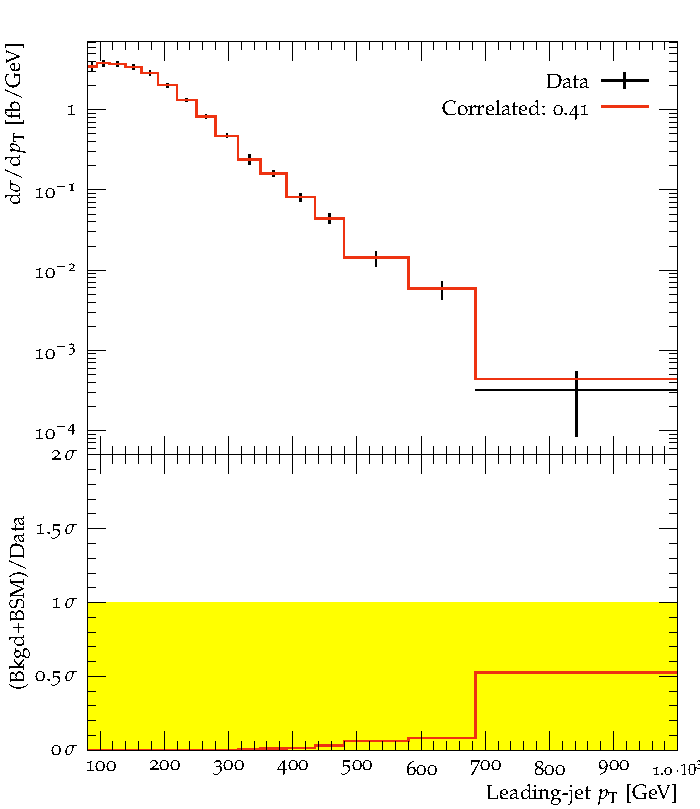
\includegraphics[width=0.36\textwidth]{Figures/VLQ/1Gen/HWZ010/Rivet/0257/d75-x01-y01}\label{fig:gen1:wjjscan:c}}
    }
    \caption{ATLAS \SI{8}{\TeV} $Wjj$ forward-lepton control region leading-jet
      \pT distributions at three points on the 95\% exclusion contour for
      $\WZH=\WZHozz$, respectively at $M_Q$ values of
      \protect\subref{fig:gen1:wjjscan:a} \unit{1000}{\GeV},
      \protect\subref{fig:gen1:wjjscan:b} \unit{1750}{\GeV}, and
      \protect\subref{fig:gen1:wjjscan:c} \unit{2250}{\GeV}. The rise and
      subsidence of a 90\% \CLs exclusion from a single $Wjj$ bin is seen as the
      contour passes from below \unit{1}{\TeV} to above \unit{2}{\TeV}.
      The black points are data, the red histogram is the VLQ contribution stacked on top of the data.
      In the lower insets, the ratio is shown and the yellow band indicates the significance, taking into
      account the statistical and systematic uncertainties on the data. The legend gives the exclusion
      (i.e. one minus the $p$-value)  for that histogram after fitting nuisance parameters for the correlated
      systematic uncertainties.}
  \label{fig:gen1:wjjscan}
\end{figure}

\subsubsection{Coupling to second-generation quarks}
The results for VLQs coupling to second-generation quarks for the four branching fraction scenarios is presented in Figure~\ref{fig:2gen:dom}. These exclusion maps scan between $\kappa=0$ and $\kappa=0.4$. The bound on the coupling is at $\kappa=0.2$ and comes from measurements of the $Z \rightarrow q\bar{q}$ couplings at LEP~\cite{Buchkremer:2013bha,ALEPH:2005ab}. Since the VLQs couple to second-generation quarks, access to valence quarks are forbidden, and the weak production diagrams of Figure~\ref{fig:feyndiags:QQ'2} and Figure~\ref{fig:feyndiags:Qq1} no longer play a dominant role. It is pair-production via the strong and electromagnetic interaction that dominates the excluded regions. In contrast to the first-generation case, only a hint of $\kappa$ dependence is visible at high $M_Q$. 

The $Z$+jets analyses are driving the exclusion in the $Z$ configuration, and the similarly the \ATLAS $WW$ analyses for the $W$ and Higgs configuration. In the $WHZ=\frac{1}{2}\frac{1}{4}\frac{1}{4}$ mixture both make an appearance. In the $M_Q$ region between \unit{1}{\TeV} and \unit{2}{\TeV}, the same emergence of the lepton+\MET{}+jet pool is present. The sensitivity is driven by the same \ATLAS VBF $Wjj$ analysis. New in the coupling to the second generation is the sensitivity coming from the \unit{13}{\TeV} \CMS jet mass analysis~\cite{Sirunyan:2018xdh} (and less so from the \ATLAS \unit{13}{\TeV} dijet and inclusive jet analysis~\cite{Aaboud:2017wsi}) beyond $M_Q=$\unit{2}{\TeV}. 

\begin{figure}[tbp]
  \centering
  \subfloat[]{
    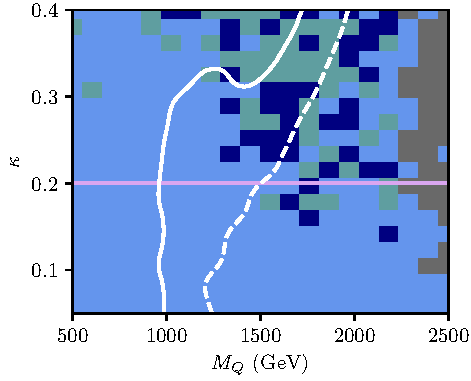
\includegraphics[width=0.45\textwidth]{Figures/VLQ/2Gen/HWZ100/dominantPools0}\label{fig:gen2:001:dom}}
  \subfloat[]{
    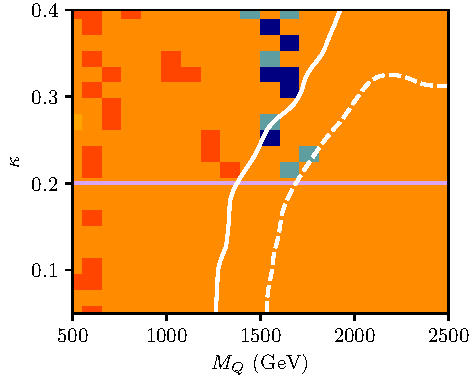
\includegraphics[width=0.45\textwidth]{Figures/VLQ/2Gen/HWZ001/dominantPools0}\label{fig:gen2:010:dom}} \\
  \subfloat[]{
    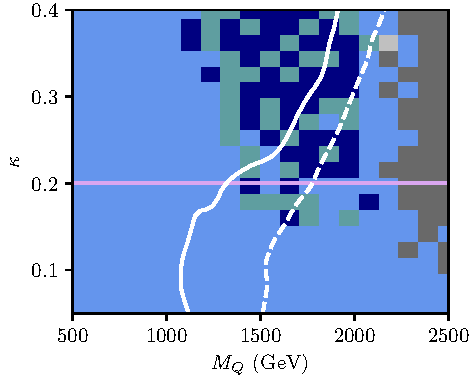
\includegraphics[width=0.45\textwidth]{Figures/VLQ/2Gen/HWZ010/dominantPools0}\label{fig:gen2:100:dom}}
  \subfloat[]{
    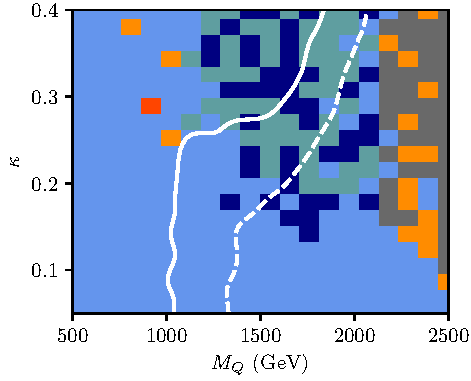
\includegraphics[width=0.45\textwidth]{Figures/VLQ/2Gen/HWZ121/dominantPools0}\label{fig:gen2:121:dom}}
  \vspace*{2ex}
  \begin{tabular}{llll}
    \swatch{cornflowerblue}~ATLAS $WW$ & \swatch{navy}~ATLAS $\mu$+\MET{}+jet & \swatch{cadetblue}~ATLAS $e$+\MET{}+jet\\
    % \swatch{snow}~ATLAS $t\bar{t}$ hadr &
    % \swatch{darkorange!90!black}~ATLAS $\mu\mu$+jet
    \swatch{orangered}~ATLAS $ee$+jet & \swatch{darkorange}~ATLAS $\mu\mu$+jet & \swatch{orange!60}~ATLAS $\ell\ell$+jet\\
    \swatch{magenta} ATLAS~4$\ell$ & \swatch{silver}~ATLAS jets & \swatch{dimgrey}~CMS jets\\
    %\swatch{gold}~ATLAS $\gamma$
  \end{tabular}
  \vspace*{2ex}
  \caption{Dominant LHC analysis pools contributing to VLQ limit-setting in the
    $\kappa$ vs VLQ mass plane, where $\kappa$ is the coupling to
    second-generation SM quarks.  All VLQ ($B, T, X, Y$) masses are set to be
    degenerate. The disfavoured regions are located above and to the left of the
    dashed (68\%~CL) and solid (95\%~CL) white contours respectively. The lower
    bounds in $\kappa$ from non-LHC flavour physics are indicated with the pink
    horizontal contour. The VLQ branching fractions to \WZH are
    \protect\subref{fig:gen2:001:dom}~\WZHzzo
    \protect\subref{fig:gen2:010:dom}~\WZHzoz
    \protect\subref{fig:gen2:100:dom}~\WZHozz and
    \protect\subref{fig:gen2:121:dom}~\WZHtoo.}
  \label{fig:2gen:dom}
\end{figure}

\subsubsection{Coupling to third-generation quarks}
Finally Figure~\ref{fig:3gen:dom} shows the exclusion in the $M_Q-\kappa$ plane for VLQs that couple only to the third-generation SM quarks. Unlike the lighter generations, no constraint exists on $\kappa$ and therefore it is scanned in the full range from $0-1$. The results are once again presented for the four $WHZ$ scenarios. Overall, pair-production dominates and $\kappa$ has little effect on the shape of the white contour. Single-production via the weak interaction is sees a further suppression in comparison to the first- and second-generation. At a high enough $\kappa$, however, the lepton+\MET{}+jet analyses sensitive to single production bring a little horizontal momentum to the white contour. 

Comparing the set of plots for the third-generation with that of the lighter generations, the biggest difference is in the $Z$ only $\xi$ configuration. For the former this region's exclusion is driven by the \ATLAS $WW$ pool (with leptons+\MET+jets signatures), with minor contributions from dilepton and four-lepton measurements, while for the latter it is driven by dilepton+jets measurements. This is a result of the allowed production and decay modes when the VLQs only couple to the top and bottom quark. For $X+q$ and $T+q$ production, there is a suppression due to the lack of top quarks in the proton sea. At high masses, $Y+q$ production dominates. Recalling from Equation~\ref{eq:vlqlagr} that the $X$ and $Y$ only couple to $W$ bosons, therefore even in the $Z$ only configuration they will decay to $W$'s. Furthermore, $Y$ and $T$ will decay to top quarks, which then decays very quickly to a $W$ boson and (usually) a bottom quark. As a result, when VLQs couple to the third-generation, there are lepton+\MET+jet signatures that are not present for the lighter generations.

It is important to highlight here the impact of analyses publishing bin-correlation information in data. The results of this section make use of correlation information where available. Correlation information allowed \Contur to use multiple bins in the $WW$ analysis pool. Without it, the (statistically limited) \ATLAS four-lepton pool would dominate a larger region of $\kappa$--$M_Q$ plane in the $Z$ only configuration, and the CMS $\ell$+\MET{}+jet analyses~\cite{Aaboud:2018uzf,Aaboud:2017fha,Aaboud:2018eki,Sirunyan:2018wem,Khachatryan:2016mnb,Sirunyan:2018ptc} would dominate the low $M_Q$ regions in the other three configurations.

\begin{figure}[tbp]
  \centering
  \subfloat[]{
    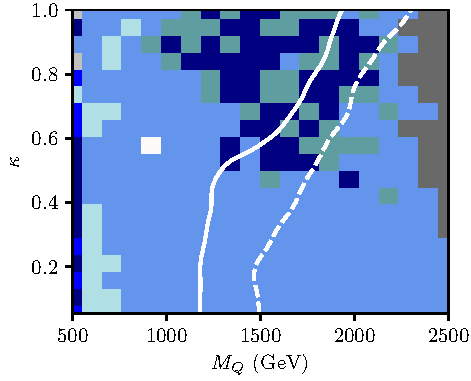
\includegraphics[width=0.45\textwidth]{Figures/VLQ/3Gen/HWZ100/dominantPools0}\label{fig:gen3:001:dom}}
  \subfloat[]{
    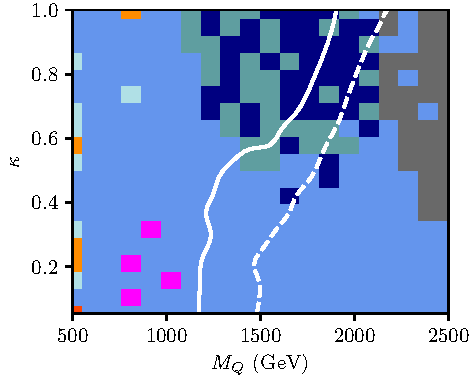
\includegraphics[width=0.45\textwidth]{Figures/VLQ/3Gen/HWZ001/dominantPools0}\label{fig:gen3:010:dom}} \\
  \subfloat[]{
    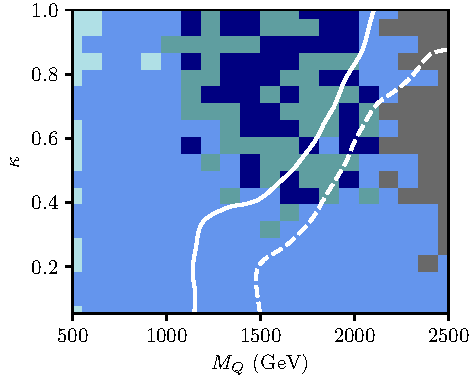
\includegraphics[width=0.45\textwidth]{Figures/VLQ/3Gen/HWZ010/dominantPools0}\label{fig:gen3:100:dom}}
  \subfloat[]{
    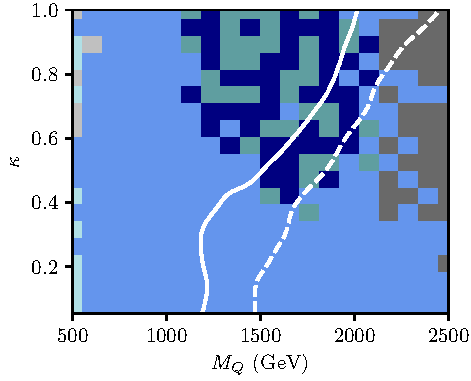
\includegraphics[width=0.45\textwidth]{Figures/VLQ/3Gen/HWZ121/dominantPools0}\label{fig:gen3:121:dom}}
  \vspace*{2ex}
  \begin{tabular}{lll}
    \swatch{cornflowerblue}~ATLAS $WW$ & \swatch{navy}~ATLAS $\mu$+\MET{}+jet & \swatch{cadetblue}~ATLAS $e$+\MET{}+jet \\
    \swatch{powderblue} CMS $\ell$+\MET{}+jet & \swatch{darkorange}~ATLAS $\mu\mu$+jet & \swatch{magenta} ATLAS~4$\ell$ \\
    \swatch{silver}~ATLAS jets & \swatch{dimgrey}~CMS jets & \swatch{snow}~ATLAS $t\bar{t}$ hadronic
  \end{tabular}
  \vspace*{2ex}
  \caption{Dominant LHC analysis pools contributing to VLQ limit-setting in the $\kappa$ vs
    VLQ mass plane, where $\kappa$ is the coupling to third-generation SM quarks.
    All VLQ ($B, T, X, Y$) masses are set to be degenerate. The disfavoured regions
    are located above and to the left of the dashed (68\%~CL)
    and solid (95\%~CL) white contours respectively. The VLQ branching
    fractions to \WZH are \protect\subref{fig:gen3:001:dom}~\WZHzzo
    \protect\subref{fig:gen3:010:dom}~\WZHzoz \protect\subref{fig:gen3:100:dom}~\WZHozz
    and \protect\subref{fig:gen3:121:dom}~\WZHtoo. %
  }
  \label{fig:3gen:dom}
\end{figure}

\subsection{Role of the \ATLAS \mFourL{} measurement}
Assuming a $\xi_Z=1$ branching fraction, the production of a vector-like $B$ or $T$ quark at the \LHC is characterized by final states with high \pT $Z$ bosons. In the case where there are two $Z$ bosons involved that both decay into charged leptons, the result is a four lepton final state made up of two same flavour, opposite sign, lepton pairs. All pair production modes can contribute to the four lepton signature since $BB$ and $TT$ decay to $ZtZt$ and $ZbZb$ respectively. Single production can also result in a four lepton final state, if the VLQ is produced in association with a $Z$ boson (Figure~\ref{fig:feyndiags:QV1} and~\ref{fig:feyndiags:QV2}). The \ATLAS \mFourL{}measurement presented in Chapter~\ref{chap:fourlepton} falls into this final state and therefore is sensitive to the production of VLQs in the $Z$ only scenario. This section explores the role that the full Run II \mFourL{} measurement plays in constraining VLQs. The results presented in the previous sections were made with \contur version 1.2.2 and \rivet 3.1.1 prior to the publication of the four lepton analysis. In this section the $Z$ only configuration scans are remade using \contur 2.1.x and \rivet 3.1.4 \todo{Differences?}, which includes the newly published four lepton measurement~\cite{m4l2021_paper}. 

\begin{figure}[tbp]
  \centering
  \subfloat[]{
    \includegraphics[width=0.55\textwidth]{Figures/VLQ/}\label{fig:gen3:001:dom}}\\
  \subfloat[]{
    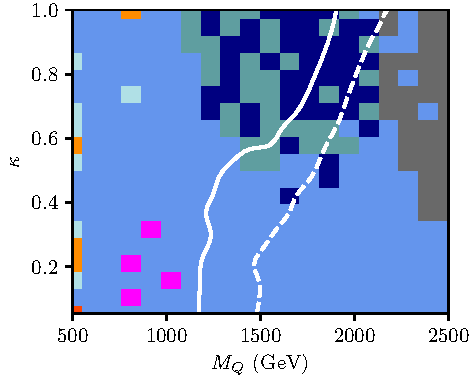
\includegraphics[width=0.55\textwidth]{Figures/VLQ/3Gen/HWZ001/dominantPools0}\label{fig:gen3:010:dom}} \\
  \subfloat[]{
    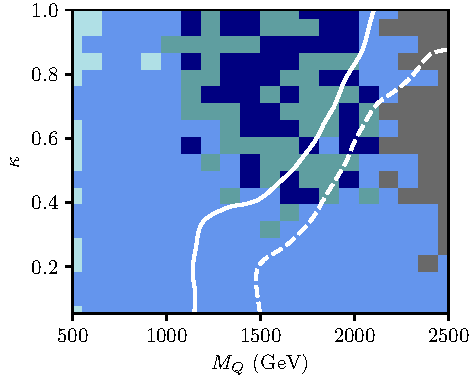
\includegraphics[width=0.55\textwidth]{Figures/VLQ/3Gen/HWZ010/dominantPools0}\label{fig:gen3:100:dom}}
  \vspace*{2ex}
  \begin{tabular}{lll}
    \swatch{cornflowerblue}~ATLAS $WW$ & \swatch{navy}~ATLAS $\mu$+\MET{}+jet & \swatch{cadetblue}~ATLAS $e$+\MET{}+jet \\
    \swatch{powderblue} CMS $\ell$+\MET{}+jet & \swatch{darkorange}~ATLAS $\mu\mu$+jet & \swatch{magenta} ATLAS~4$\ell$ \\
    \swatch{silver}~ATLAS jets & \swatch{dimgrey}~CMS jets & \swatch{snow}~ATLAS $t\bar{t}$ hadronic
  \end{tabular}
  \vspace*{2ex}
  \caption{Dominant LHC analysis pools contributing to VLQ limit-setting in the $\kappa$ vs
    VLQ mass plane, where $\kappa$ is the coupling to third-generation SM quarks.
    All VLQ ($B, T, X, Y$) masses are set to be degenerate. The disfavoured regions
    are located above and to the left of the dashed (68\%~CL)
    and solid (95\%~CL) white contours respectively. The VLQ branching
    fractions to \WZH are \protect\subref{fig:gen3:001:dom}~\WZHzzo
    \protect\subref{fig:gen3:010:dom}~\WZHzoz \protect\subref{fig:gen3:100:dom}~\WZHozz
    and \protect\subref{fig:gen3:121:dom}~\WZHtoo. %
  }
  \label{fig:3gen:dom}
\end{figure}
